%\documentclass[handout]{beamer}
\documentclass{beamer}

\mode<presentation>
{
\usetheme{default}
\usefonttheme[onlymath]{serif}
%\usetheme{Singapore}
%\usetheme{Warsaw}
%\usetheme{Malmoe}
% \useinnertheme{circles}
% \useoutertheme{infolines}
% \useinnertheme{rounded}

\setbeamercovered{transparent=5}
}

\usepackage[english]{babel}
\usepackage[latin1]{inputenc}
\usepackage{textpos,alltt,listings,multirow,ulem,siunitx}
\newcommand\hmmax{0}
\newcommand\bmmax{0}
\usepackage{bm}

% font definitions, try \usepackage{ae} instead of the following
% three lines if you don't like this look
\usepackage{mathptmx}
\usepackage[scaled=.90]{helvet}
%\usepackage{courier}
\usepackage[T1]{fontenc}
\usepackage{tikz}
\usetikzlibrary[shapes,shapes.arrows,arrows,shapes.misc,fit,positioning]

% \usepackage{pgfpages}
% \pgfpagesuselayout{4 on 1}[a4paper,landscape,border shrink=5mm]

\usepackage{slashbox,multirow,listings,booktabs}
\usepackage{xspace}
\makeatletter
\DeclareRobustCommand\onedot{\futurelet\@let@token\@onedot}
\def\@onedot{\ifx\@let@token.\else.\null\fi\xspace}
\def\eg{{e.g}\onedot} \def\Eg{{E.g}\onedot}
\def\ie{{i.e}\onedot} \def\Ie{{I.e}\onedot}
\def\cf{{c.f}\onedot} \def\Cf{{C.f}\onedot}
\def\etc{{etc}\onedot}
\def\vs{{vs}\onedot}
\def\wrt{w.r.t\onedot}
\def\dof{d.o.f\onedot}
\def\etal{{et al}\onedot}
\makeatother

\usepackage{tikz}
\usetikzlibrary[shapes,shapes.arrows,arrows,shapes.misc,fit,positioning]

\usepackage{siunitx}
\DeclareSIUnit\year{a}
\DeclareSIUnit\byte{B}
\sisetup{retain-unity-mantissa = false}

\usepackage{fancyvrb}
\usepackage{minted}
\newminted{c}{gobble=2}
\newminted{python}{gobble=2}
%\newmint[cverb]{c}{} 
\newcommand\cverb[1][]{\SaveVerb[%
    aftersave={\textnormal{\UseVerb[#1]{vsave}}}]{vsave}}
\newcommand\cfunc[1][]{\SaveVerb[%
    aftersave={\textnormal{\UseVerb[#1]{vsave}\texttt{()}}}]{vsave}}
\newcommand\pyverb[1][]{\SaveVerb[%
    aftersave={\textnormal{\UseVerb[#1]{vsave}}}]{vsave}}
\def\asm#1{{\tt #1}}
\def\code#1{{\tt #1}}
\def\shell#1{{\tt \$ #1}}

\newcommand\email[1]{{\href{mailto:#1}{\nolinkurl{#1}}}}

\newcommand{\II}{\mathcal{I}}
\newcommand{\C}{\mathbb{C}}
\newcommand{\D}{\mathcal{D}}
\newcommand{\EE}{\mathcal{E}}
\newcommand{\F}{\mathcal{F}}
\newcommand{\I}{\mathcal{I}}
\newcommand{\N}{\mathcal{N}}
\newcommand{\PP}{\mathcal{P}}
\newcommand\Ppc{\ensuremath{\mathsf P}}
\newcommand{\bigO}{\ensuremath{\mathcal{O}}}
\newcommand{\R}{\mathbb{R}}
\newcommand{\Rz}{\mathcal{R}}
\newcommand{\QQ}{\mathcal Q}
\newcommand{\VV}{\mathcal V}
\newcommand{\ASM}{\mathrm{ASM}}
\newcommand{\RASM}{\mathrm{RASM}}

\newcommand{\kb}{\tt}
\newcommand{\Pk}[1]{\ensuremath{P_{#1}}}
\newcommand{\Qk}[1]{\ensuremath{Q_{#1}}}
\newcommand{\Pkdisc}[1]{\ensuremath{P_{#1}^{\text{disc}}}}
\newcommand{\Qkdisc}[1]{\ensuremath{Q_{#1}^{\text{disc}}}}
\newcommand{\blue}{\textcolor{blue}}
\newcommand{\green}{\textcolor{green!70!black}}
\newcommand{\red}{\textcolor{red}}
\newcommand{\brown}{\textcolor{brown}}
\newcommand{\cyan}{\textcolor{cyan}}
\newcommand{\magenta}{\textcolor{magenta}}
\newcommand{\yellow}{\textcolor{yellow}}
\newcommand{\mini}{\mathop{\rm minimize}}
\newcommand{\st}{\mbox{subject to }}
\newcommand{\lap}{\Delta}
\newcommand{\grad}{\nabla}
\newcommand\mtab{\hspace{\stretch{1}}}
\newcommand\ud{\,\mathrm{d}}
\newcommand\bslash{{$\backslash$}}
\newcommand\half{{\frac 1 2}}
\newcommand{\abs}[1]{\left\lvert #1 \right\rvert}
\newcommand{\bigabs}[1]{\big\lvert #1 \big\rvert}
\newcommand{\norm}[1]{\left\lVert #1 \right\rVert}
\newcommand\oneitem[1]{\begin{itemize} \item #1 \end{itemize}}
\newcommand\pfrak{{\mathfrak p}}
\newcommand\nfrak{{\mathfrak n}}
\newcommand\ff{\bm f}
\newcommand\mm{\bm m}
\newcommand\nn{\bm n}
\newcommand\uu{\bm u}
\newcommand\vv{\bm v}
\newcommand\ww{\bm w}
\newcommand\DD{D}
\newcommand{\tcolon}{\!:\!}
\DeclareMathOperator{\sgn}{sgn}
\DeclareMathOperator{\card}{card}
\DeclareMathOperator{\trace}{tr}
\DeclareMathOperator{\erf}{erf}
\DeclareMathOperator{\sspan}{span}
\renewcommand{\bar}{\overline}
% \DeclareMathOperator{\divergence}{div}
% \renewcommand\div\divergence
\renewcommand{\div}{{\nabla \cdot}}
\newcommand\spliceop{\leftrightsquigarrow}
\newcommand\splice[5]{{#1} \overset{#5}{\underset{#3,#4}{\leftrightsquigarrow}} {#2}}
\newcommand{\ip}[2]{{\left\langle #1, #2 \right\rangle}}
\newcommand{\Linfty}{{L^\infty}}

% Dimensionless numbers
\newcommand{\Peclet}{{\mathrm{Pe}}}
\newcommand{\Reynolds}{{\mathrm{Re}}}
\newcommand{\Rayleigh}{{\mathrm{Ra}}}
\newcommand{\Mach}{{\mathrm{Ma}}}
\newcommand{\Prandtl}{{\mathrm{Pr}}}
\newcommand{\Grashof}{{\mathrm{Gr}}}

\newcommand{\PETSc}{{PETSc}}
\newcommand{\Dohp}{{Dohp}}
\newcommand\libmesh{\texttt{libMesh}}
\newcommand\dealii{\texttt{Deal.II}}
\newcommand\MatMult{\cverb|MatMult|}
\newcommand\MatSolve{\cverb|MatSolve|}
\newcommand{\secref}[1]{{Section~\ref{#1}}}
\newcommand{\chapref}[1]{{Chapter~\ref{#1}}}
\newcommand{\figref}[1]{{Figure~\ref{#1}}}
\newcommand{\tabref}[1]{{Table~\ref{#1}}}
\newcommand\AIJ{{\cverb|AIJ|}}
\newcommand\AIJInode{\cverb|AIJ|/\cverb|Inode|}
\newcommand\BAIJ[1][]{\ifthenelse{\equal{#1}{}}{\cverb|BAIJ|}{\ensuremath{\cverb|BAIJ|(#1)}}}
\newcommand\SBAIJ[1][]{\ifthenelse{\equal{#1}{}}{\cverb|SBAIJ|}{\ensuremath{\cverb|SBAIJ|(#1)}}}
\newcommand\todo[1]{{\color{red}\bf [TODO: #1]}}
\newcommand\tf[1]{\hat{#1}}     % test functions


\title{A Software Framework in Python for Generating Optimal Isogeometric Kernels on the PowerPC 450}

\author{Aron Ahmadia\inst{1}, \emph{Jed Brown}\inst{2}, Nathan Collier\inst{1}, Tareq Malas\inst{1}, John Gunnels\inst{3}}


% - Use the \inst command only if there are several affiliations.
% - Keep it simple, no one is interested in your street address.
\institute[ANL]
{
  \inst{1}{King Abdullah University of Science and Technology}\and
  \inst{2}{Argonne National Laboratory} / {ETH Z\"urich}\and
  \inst{3}{IBM Watson}
}

\date{2011-07-13}

% This is only inserted into the PDF information catalog. Can be left
% out.
\subject{Talks}


% If you have a file called "university-logo-filename.xxx", where xxx
% is a graphic format that can be processed by latex or pdflatex,
% resp., then you can add a logo as follows:

% \pgfdeclareimage[height=0.5cm]{university-logo}{university-logo-filename}
% \logo{\pgfuseimage{university-logo}}



% Delete this, if you do not want the table of contents to pop up at
% the beginning of each subsection:
% \AtBeginSubsection[]
% {
% \begin{frame}<beamer>
% \frametitle{Outline}
% \tableofcontents[currentsection,currentsubsection]
% \end{frame}
% }

% If you wish to uncover everything in a step-wise fashion, uncomment
% the following command:

%\beamerdefaultoverlayspecification{<+->}

\begin{document}
\lstset{language=C}
\normalem

\begin{frame}
\titlepage
\end{frame}

\begin{frame}{Blue Gene/P}
    \begin{quote}\large \centering
    The easiest way to make software scalable \\
    is to make it sequentially inefficient. \\
    (Gropp 1999)
  \end{quote}

  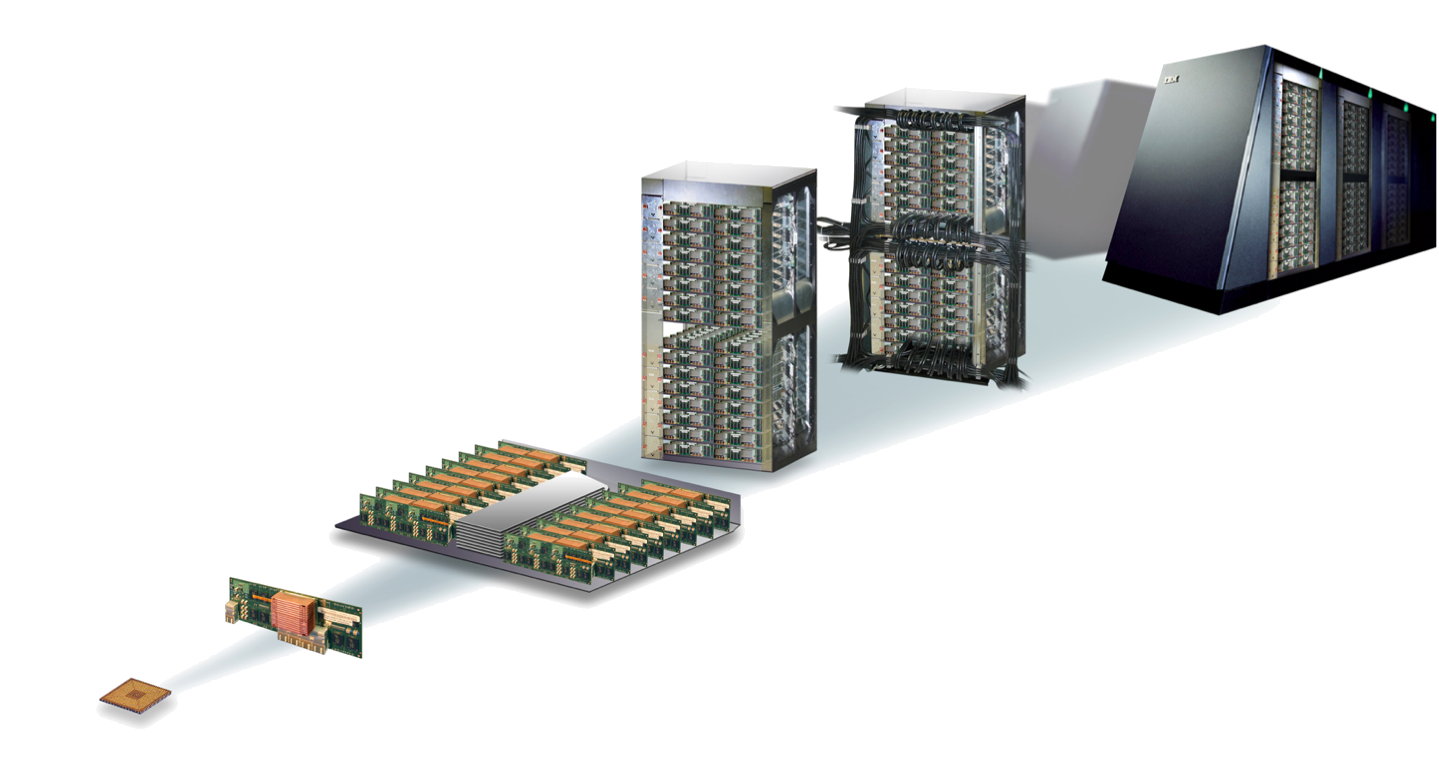
\includegraphics[width=\textwidth]{figures/BlueGenePRacks}
\end{frame}
\begin{frame}{Blue Gene/P}
  \begin{columns}
    \begin{column}{0.6\textwidth}
      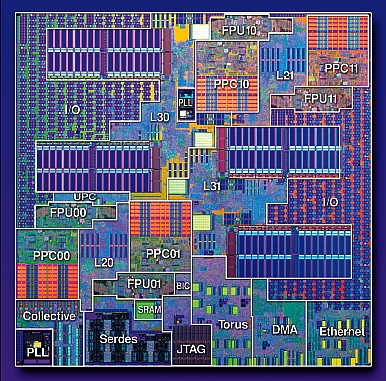
\includegraphics[width=\textwidth]{figures/BlueGenePDie}
    \end{column}
    \begin{column}{0.4\textwidth}
      \begin{itemize}
      \item 4 cores @ 850 Mhz
      \item 32 16-bytes FP registers
      \item 1 packed FMA per cycle, latency 5
      \item 0.5 load per cycle, latency 4
      \item 3 memory requests in-flight
      \item write-through cache, FIFO eviction policy
      \item up to 5 memory streams
      \end{itemize}
    \end{column}
  \end{columns}
\end{frame}

\begin{frame}{What makes compiled code slow?}
  \begin{block}{Compilers are bad at}
    \begin{itemize}
    \item SIMD instructions
    \item Alignment constraints
    \item Register allocation
    \item Scheduling for out-of-order execution
    \item Transformations to reduce memory bandwidth
    \end{itemize}
  \end{block}
  \begin{block}{But it's not hopeless}
    \begin{itemize}
    \item BG/P has rich SIMD instructions
    \item Large kernels reuse small kernels
    \item Register allocation usually has a pattern
    \end{itemize}
  \end{block}
\end{frame}

\begin{frame}{Code generation}
  \begin{block}{Mako templates writing inline assembly}
    \begin{itemize}
    \item Easy to control unrolling and jamming
    \item Hard to manage generators with complex control flow
    \item Hard to keep track of register names and debug
    \item How to manage in-order execution?
    \item Smells bad
    \end{itemize}
  \end{block}
  \begin{block}{SimASM: All Python}
    \begin{itemize}
    \item Name some or all registers, can mix pinned and unpinned registers
    \item Build kernel using generators/loops/objects/etc
    \item Transform to partial order according to instruction dependencies (hazards)
    \item Transform/traverse using simulator, can debug correctness too
    \item Hazards that cause stalls are shown and explained
    \end{itemize}
  \end{block}
\end{frame}

\begin{frame}[fragile,shrink=5]{Instruction Set}
\begin{align*}
  t_p &\gets a_s c_s + b_p \\
  t_s &\gets a_s c_p + b_s
\end{align*}
\begin{minted}{python}
class fxcxma(Instruction):
  def __init__(self,rt,ra,rc,rb):
    Instruction.__init__(self)
    self.save(locals(),'rt ra rc rb')
    self.reads(ra,rc,rb)
    self.writes(rt)
    self.uses(PPC.FP,5)
  def run(self,c):
    ra,rc,rb = c.access_fpregisters(self.ra,self.rc,self.rb)
    c.fp[self.rt] = FPVal(ra.s*rc.s + rb.p,
                          ra.s*rc.p + rb.s)
\end{minted}
\end{frame}


\begin{frame}{Stencil Operation}
  \centering
  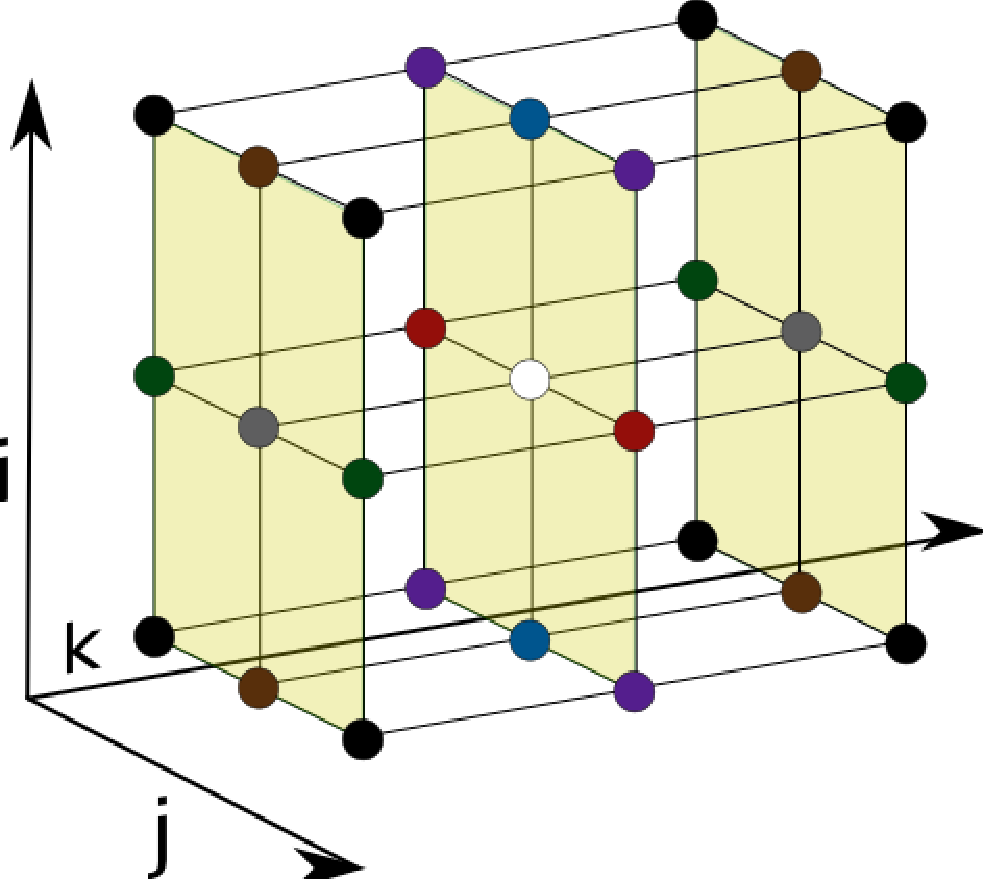
\includegraphics[width=0.6\textwidth]{figures/27_point_colored}
  \begin{itemize}
  \item Cartesian grid, constant coefficient scalar PDE.
  \item Forward propagation operator or Jacobi smoother.
  \item Memory bandwidth limited? (Datta \etal 2009, SIAM Review)
    \begin{itemize}
    \item Cache blocking: 26 Mstencil/s (41\% of theoretical 63 at FPU peak)
    \end{itemize}
  \item Load/store and FPU limited?
    \begin{itemize}
    \item Jamming and SIMD: 93\% in L1, 70\% from DRAM
    \end{itemize}
  \end{itemize}
\end{frame}

\begin{frame}
  \centering
  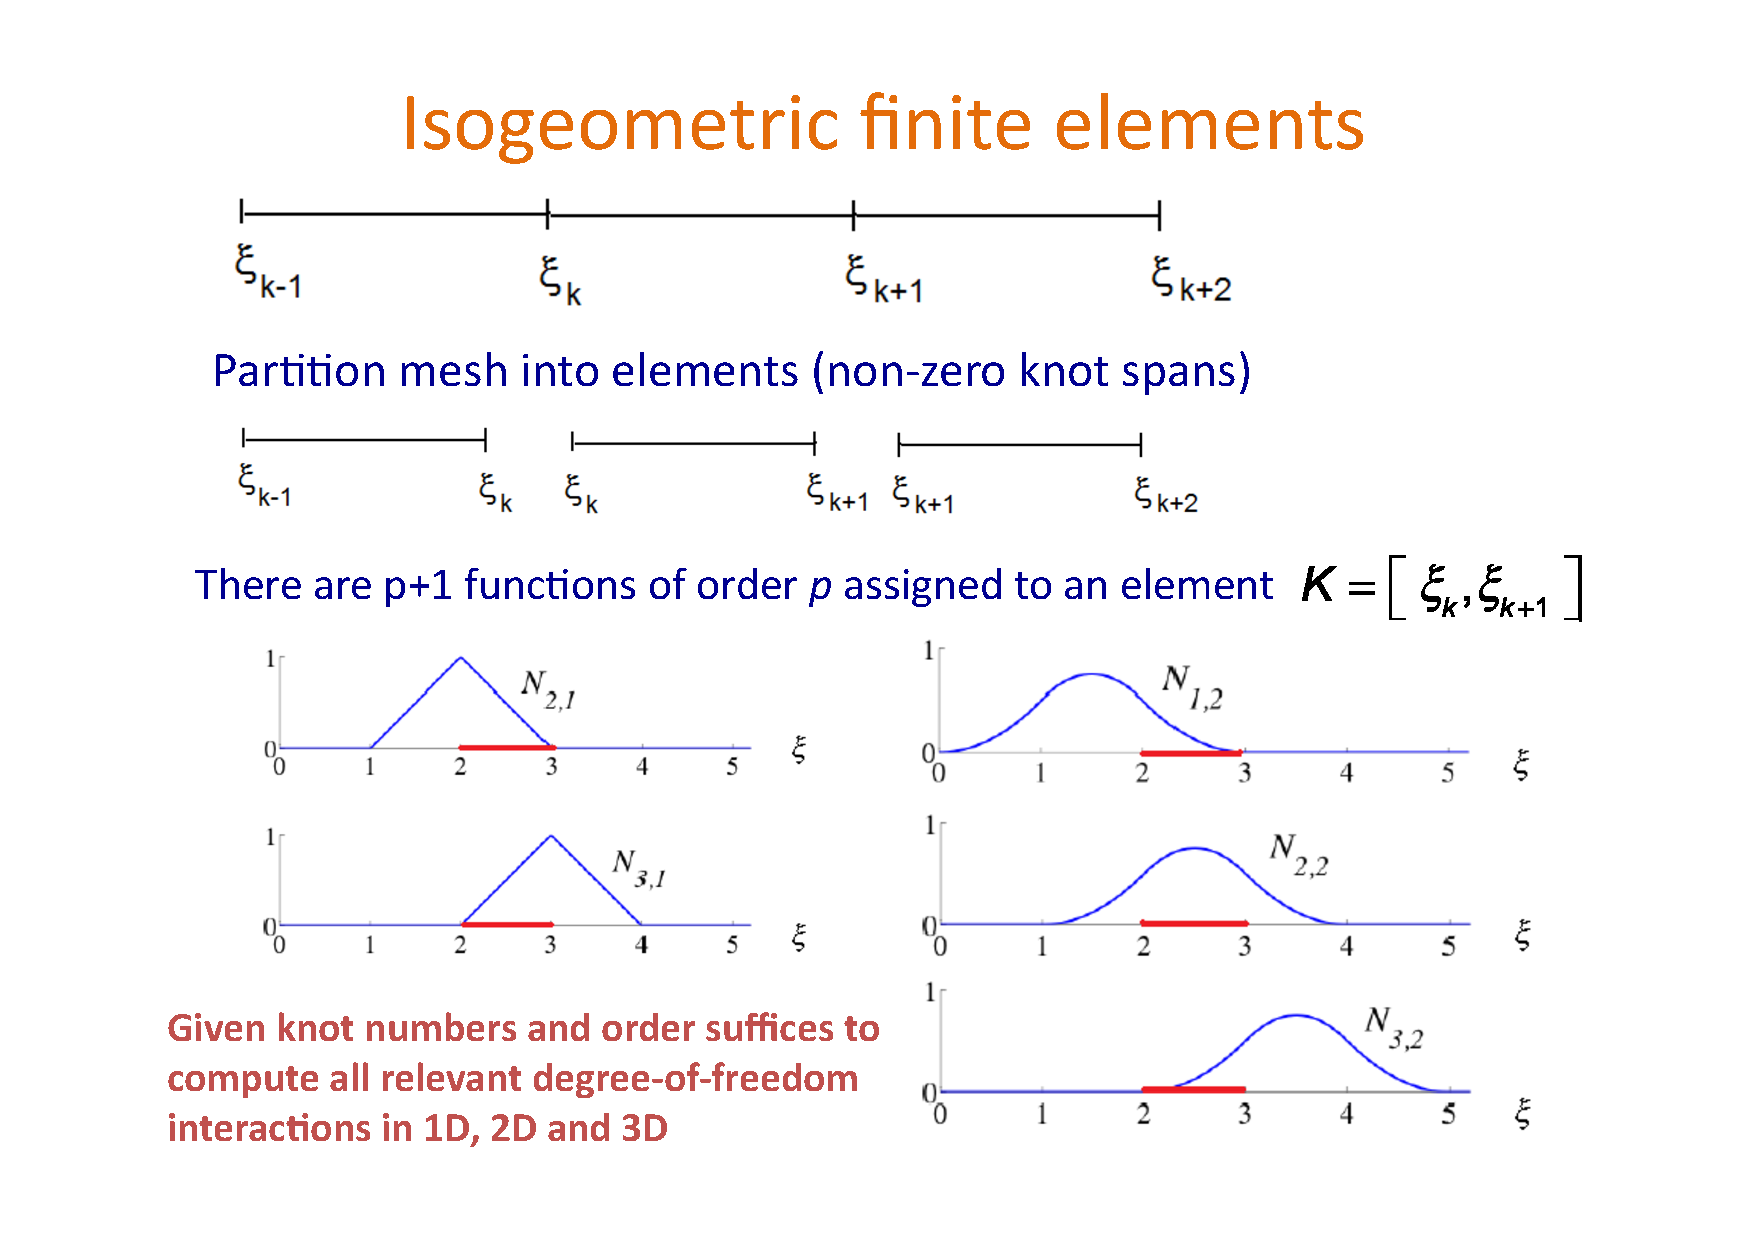
\includegraphics[width=1.1\textwidth]{figures/IGACalo}
%  (c/o Victor Calo)
\end{frame}

\begin{frame}{IGA compared to standard FEM}
  \begin{itemize}
  \item Can exactly conform to some engineering geometries.
  \item Better impedence match with solid modeling (CAD).
  \item Fewer degrees of freedom for 4th order problems,\\
    \quad \eg no rotation dofs for shells.
  \item More nonzeros per row as continuity is increased.
  \item More quadrature points per dof (higher arithmetic intensity).
  \item Needs logically structured grids \\
    (T-splines can join structured patches)
  \item All-positive basis functions useful for some problems \\
    (maintain positivity, robust conservative normals)
  \item Non-interpolatary basis can be tricky for preconditioning.
  \end{itemize}
\end{frame}

\begin{frame}
  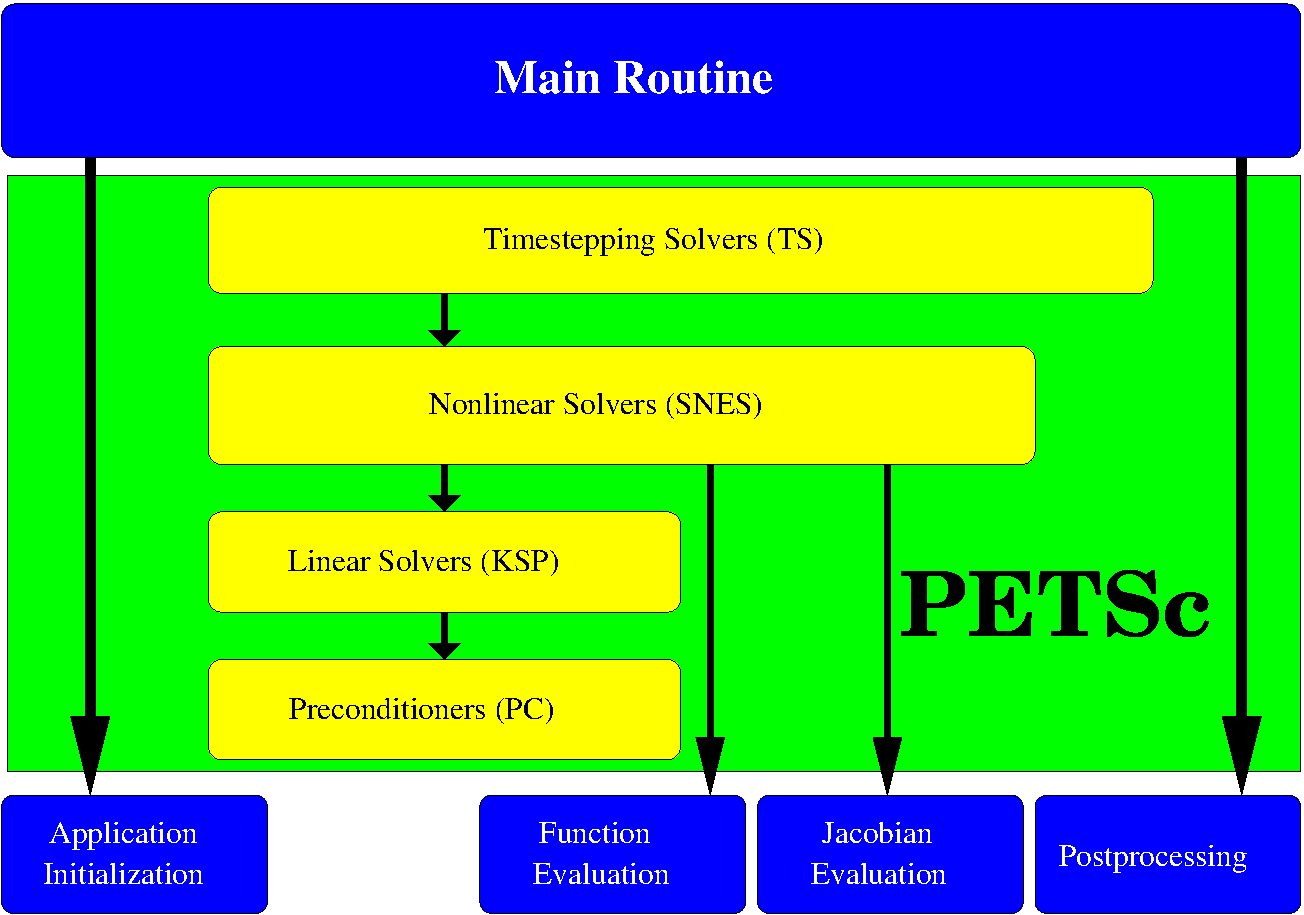
\includegraphics[width=0.8\textwidth]{figures/SNES/FlowControl}
  \begin{itemize}
  \item IGA used to evaluate nonlinear residuals
  \item PETSc \cverb|DA| used to manage parallelism.
  \item Adaptive time integration using method of lines.
    \begin{itemize}
    \item Generalized $\alpha$ method from PETSc \cverb|TS|.
    \end{itemize}
  \item Matrix-free Newton-Krylov, need only residuals for implicit solve.
  \end{itemize}
\end{frame}

% \begin{frame}{Cahn-Hilliard Equation}
%   Models phase separation: find concentration $c$
%   \begin{equation*}
%     \ip{w}{\frac{\partial c}{\partial t}}_\Omega + \ip{\nabla w}{M(c)\nabla\mu(c) + \nabla M(c)\Delta c}_\Omega + \ip{\Delta w}{M(c) \Delta c}_\Omega = 0 \quad \forall w
%   \end{equation*}
%   Boundary conditions and equations of state $\mu(c)$ and $M(c)$.
%   \begin{minted}[gobble=4]{c}
%     R_rho  = Na*rho_t;
%     R_rho += -rho*(Na_x*ux + Na_y*uy);

%     R_ux  = Na*ux*rho_t;
%     R_ux += Na*rho*ux_t;
%     R_ux += -rho*(Na_x*ux*ux + Na_y*ux*uy);
%     R_ux += -Na_x*p;
%     R_ux += rRe*(Na_x*tau_xx + Na_y*tau_xy);
%     R_ux += -Ca2*rho*(Na_xx*rho_x + Na_xy*rho_y);
%     R_ux += -Ca2*Na_x*(rho_x*rho_x + rho_y*rho_y);
%     R_ux += -Ca2*Na*(rho_xx*rho_x + rho_xy*rho_y);
%     R_ux += -Ca2*rho_x*(Na_x*rho_x + Na_y*rho_y);
%   \end{minted}
% \end{frame}

\begin{frame}[fragile,shrink=5]{Navier-Stokes Korteweg}
  Phase field model for water/water vapor two-phase flows.
  Find $U = (\rho,\uu)$ such that $B(W,U) = 0$ for all $W = (q,\ww)$, plus boundary conditions.
  \begin{equation*}
    \begin{split}
      B(W,U) &= \int_\Omega q \frac{\partial \rho}{\partial t} - \nabla q\cdot \rho\uu
      + w\cdot \left[\uu\frac{\partial\rho}{\partial t} + \rho\frac{\partial \uu}{\partial t} \right] \\
      &+ \nabla w \tcolon \Big[ -\rho\uu\otimes\uu + \tau - (p + \lambda \abs{\nabla \rho}^2)\bm 1 \Big] \\
      &- \nabla(\nabla\cdot\ww)\cdot \lambda\rho\nabla\rho - \nabla(\nabla\rho\cdot\ww)\cdot\lambda\nabla\rho = 0
    \end{split}
  \end{equation*}
  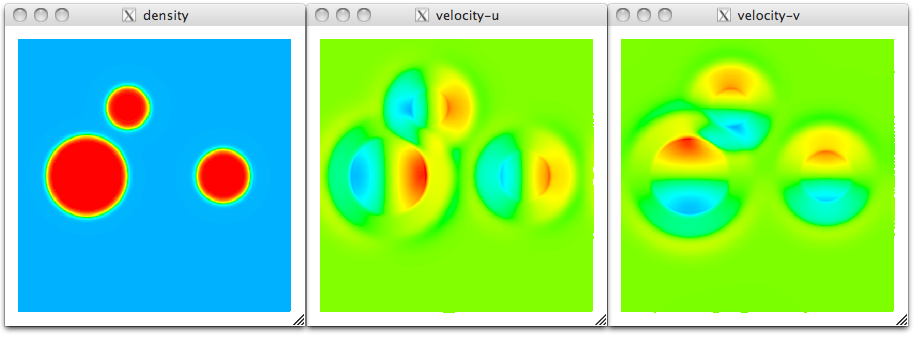
\includegraphics[width=\textwidth]{figures/NSK}
\end{frame}

\begin{frame}[fragile,shrink=5]{Navier-Stokes Korteweg}
  Phase field model for water/water vapor two-phase flows.
  Find $U = (\rho,\uu)$ such that $B(W,U) = 0$ for all $W = (q,\ww)$, plus boundary conditions.
  \begin{equation*}
    \begin{split}
      B(W,U) &= \int_\Omega q \frac{\partial \rho}{\partial t} - \nabla q\cdot \rho\uu
      + w\cdot \left[\uu\frac{\partial\rho}{\partial t} + \rho\frac{\partial \uu}{\partial t} \right] \\
      &+ \nabla w \tcolon \Big[ -\rho\uu\otimes\uu + \tau - (p + \lambda \abs{\nabla \rho}^2))\bm 1 \Big] \\
      &- \nabla(\nabla\cdot\ww)\cdot \lambda\rho\nabla\rho - \nabla(\nabla\rho\cdot\ww)\cdot\lambda\nabla\rho = 0
    \end{split}
  \end{equation*}
  \begin{minted}[gobble=2]{c}
  for each Na,Na_x,Na_xx,Na_y,Na_yy: // test functions
    R_rho  = Na*rho_t;
    R_rho += -rho*(Na_x*ux + Na_y*uy);
    R_ux  = Na*ux*rho_t;
    R_ux += Na*rho*ux_t;
    R_ux += -rho*(Na_x*ux*ux + Na_y*ux*uy);
    R_ux += -Na_x*p;
    R_ux += rRe*(Na_x*tau_xx + Na_y*tau_xy);
    R_ux += -Ca2*rho*(Na_xx*rho_x + Na_xy*rho_y);
    ...
  \end{minted}
\end{frame}

\begin{frame}[fragile]{Transform to more vector-friendly form}
  \begin{itemize}
  \item Pre-compute ``physics'' \cverb|W| at each quadrature point
  \item assembling the residual becomes dot products
  \begin{minted}[gobble=2]{c}
  for each Na,Na_x,Na_xx,Na_y,Na_yy:
    R_rho  = Na*W[irho_t];
    R_rho += Na_x*W[rho_nax];
    R_rho += Na_y*W[rho_nay];
    R_ux  = Na*W[ux_na];
    R_ux += Na_x*W[ux_nax];
    R_ux += Na_y*W[ux_nay];
    R_ux += Na_xx*W[u_naxx];
    R_ux += Na_xy*W[u_naxy];
  \end{minted}
  \item 1.9x speedup
  \end{itemize}
\end{frame}

\begin{frame}[fragile]{Vectorize using SimASM}
  \begin{itemize}
  \item Define context-sensitive vector primitives
    \begin{minted}[gobble=4]{python}
      def muladd_copy(self, com, rt, ra, rb):
        if ra[1] == 0:
          return isa.fxcpmadd(rt,com.W[ra[0]],rb,rt)
        else:
          return isa.fxcsmadd(rt,com.W[ra[0]],rb,rt)
    \end{minted}
  \item Unrolled/jammed vector assembly looks ``close'' to the physics
    \begin{minted}[gobble=4]{python}
      [self.muladd_copy(com, 'R_rho', com.rho_nax, 'Na_x'),
      self.muladd_copy(com, 'R_ux', com.ux_nax, 'Na_x'),
      self.muladd_copy(com, 'R_uy', com.uy_nax, 'Na_x')]
    \end{minted}
  \item Still limited by load/store unit.
  \item Multiple quadrature points and elements could amortize load/store cost.
  \item More clever transformations?
  \item Still need to optimize computation of coordinate transformation for high end-to-end throughput.
  \end{itemize}
\end{frame}


\begin{frame}{Perspective on SimASM}
  \begin{block}{Blue Gene/P is representative of future architectures}
    \begin{itemize}
    \item In-order execution
    \item Longer FP registers
    \item More cores
    \item Less memory bandwidth
    \end{itemize}
  \end{block}
  \begin{block}{Need some way to get close to peak performance}
    \begin{itemize}
    \item SSE intrinsics are pretty good on Intel/AMD
      \begin{itemize}
      \item Better designed intrinsic API
      \item Out of order execution more tolerant
      \item Fewer registers
      \item Lightweight templating (\eg Mako) might be good enough
      \end{itemize}
    \item Interesting alternatives
      \begin{itemize}
      \item OpenCL (wide vectorization, different memory model)
      \item Intel SPMD Program Compiler (\url{ispc.github.com})
      \end{itemize}
    \end{itemize}
  \end{block}
\end{frame}

\begin{frame}{Outlook}
  \begin{block}{Lots more to do with IGA/FEM}
    \begin{itemize}
    \item Library interface for vectorized physics/assembly
    \item Connecting structured blocks (T-splines)
    \item Algorithmic (analytic Jacobians, preconditioning)
    \end{itemize}
  \end{block}
  \begin{block}{SimASM}
    \begin{itemize}
    \item Better optimization framework.
    \item Different target architectures (\eg Blue Gene/Q, Knight's Corner).
    \item Interface improvements/visualization.
    \item Code generation from high level/symbolic description?
    \item \url{bitbucket.org/jedbrown/simasm}
    \end{itemize}
  \end{block}
\end{frame}

\end{document}
